\documentclass[11pt,fleqn]{article}
\usepackage[margin=1in,top=1in,bottom=1in]{geometry}
\usepackage{tikz}
\usepackage{mathtools}
\usepackage{longtable}
\usepackage{enumitem}
\usepackage[hidelinks]{hyperref}
%\usepackage[dvips]{graphics}
%\usepackage[table]{xcolor}
%\usepackage{amssymb}
\usepackage{float}
%\usepackage{subfig}
\usepackage{booktabs}
\usepackage{subcaption}

\usepackage[normalem]{ulem}

\usepackage{multicol}
\usepackage{txfonts}
\usepackage{amsfonts}
\usepackage{natbib}
\usepackage{gb4e}
\usepackage[all]{xy}
\usepackage{rotating}
\usepackage{tipa}
\usepackage{multirow}
\usepackage{authblk}
\usepackage{url}
\usepackage{pdflscape}
\usepackage{rotating}
\usepackage{adjustbox}
\usepackage{array}


\def\bad{{\leavevmode\llap{*}}}
\def\marginal{{\leavevmode\llap{?}}}
\def\verymarginal{{\leavevmode\llap{??}}}
\def\swmarginal{{\leavevmode\llap{4}}}
\def\infelic{{\leavevmode\llap{\#}}}

\definecolor{airforceblue}{rgb}{0.36, 0.54, 0.66}
%\definecolor{gray}{rgb}{0.36, 0.54, 0.66}

\definecolor{Pink}{RGB}{240,0,120}
\newcommand{\red}[1]{\textcolor{Pink}{#1}}
\newcommand{\jd}[1]{\textbf{\textcolor{Pink}{[jd: #1]}}}
\definecolor{green}{RGB}{0,158,115}
\definecolor{orange}{RGB}{213,94,0}

\newcommand{\dashrule}[1][black]{%
  \color{#1}\rule[\dimexpr.5ex-.2pt]{4pt}{.4pt}\xleaders\hbox{\rule{4pt}{0pt}\rule[\dimexpr.5ex-.2pt]{4pt}{.4pt}}\hfill\kern0pt%
}

\setlength{\parindent}{.3in}
\setlength{\parskip}{0ex}

\newcommand{\yi}{\'{\symbol{16}}}
\newcommand{\nasi}{\~{\symbol{16}}}
\newcommand{\hina}{h\nasi na}
\newcommand{\ina}{\nasi na}

\newcommand{\foc}{$_{\mbox{\small F}}$}

\hyphenation{par-ti-ci-pa-tion}

\setlength{\bibhang}{0.5in}
\setlength{\bibsep}{0mm}
\bibpunct[:]{(}{)}{,}{a}{}{,}

\newcommand{\6}{\mbox{$[\hspace*{-.6mm}[$}} 
\newcommand{\9}{\mbox{$]\hspace*{-.6mm}]$}}
\newcommand{\sem}[2]{\6#1\9$^{#2}$}
\renewcommand{\ni}{\~{\i}}

\newcommand{\citepos}[1]{\citeauthor{#1}'s \citeyear{#1}}
\newcommand{\citeposs}[1]{\citeauthor{#1}'s}
\newcommand{\citetpos}[1]{\citeauthor{#1}'s (\citeyear{#1})}

\newcolumntype{R}[2]{%
    >{\adjustbox{angle=#1,lap=\width-(#2)}\bgroup}%
    l%
    <{\egroup}%
}
\newcommand*\rot{\multicolumn{1}{R{90}{0em}}}% no optional argument here, please!


\title{I don't know if projection is binary. \\ Did \citealt{mandelkern-etal2020} discover that it is?}

\author[$\circ$]{Judith Tonhauser}
\author[$\bullet$]{Judith Degen}
\affil[$\circ$]{University of Stuttgart}
\affil[$\bullet$]{Stanford University}

\renewcommand\Authands{ and }

\newcommand{\jt}[1]{\textbf{\color{blue}JT: #1}}

\begin{document}

\maketitle


\begin{abstract}

Presuppositions are taken to typically project out of entailment-canceling environments like the scope of negation (e.g., \citealt{frege1892,ccmg90}). While projection is often characterized as binary (that is, content either typically projects or not), there is mounting empirical evidence that projection is gradient, with content being more or less projective (e.g., \citealt{karttunen71b,xue-onea11,demarneffe-etal-sub23,tbd-variability,degen-tonhauser-language}). \citealt{mandelkern-etal2020} critically evaluated the inference rating measures on which this empirical evidence is based and proposed that naturalness ratings in explicit ignorance contexts are more suitable to measure binary projection and, thereby, to distinguish presupposition triggers from nontriggers. This paper presents the results of an experiment designed to investigate whether the measure proposed by \citealt{mandelkern-etal2020} can distinguish factive predicates (presumed presupposition triggers) from nonfactive ones (nontriggers). While the results do not support \citepos{mandelkern-etal2020} hypothesis and are rather in line with results based on inference rating measures (e.g., \citealt{degen-tonhauser-language}), the results suggest that naturalness ratings in explicit ignorance contexts are sensitive to felicity conditions of anaphoric projective content.

\end{abstract}

\bigskip

\noindent
{\bf Keywords:} Presuppositions, binary vs.\ gradient projection, inference ratings, naturalness ratings in explicit ignorance contexts. 

\bigskip

\noindent
{\bf Acknowledgments:} 

\noindent
For helpful comments on this project we thank Craige Roberts, Gregory Scontras, and Mandy Simons.

\newpage
		
\section{Introduction}\label{s1}

Presuppositions are defined as content that typically projects out of entailment-canceling environments, like the scope of negation or a polar interrogative (e.g., \citealt{frege1892,ccmg90}).\footnote{Conventional implicatures also project out of these environments. They differ from presuppositions in that they contribute novel information. For discussion see, e.g., \citealt{ccmg90,potts05}.} Thus, a content like the content of the clausal complement (CC) of {\em know} in (\ref{first}a) is taken to be a presupposition because a speaker who utters (\ref{first}a) is typically taken to believe the CC, that Julian dances salsa, even though the clausal complement occurs in a polar interrogative. By contrast, the CC of {\em think} in (\ref{first}b) is not assumed to be a presupposition because it does not typically project. Accordingly, {\em know} is analyzed as a presupposition trigger, but {\em think} is not.

\begin{exe}
\ex\label{first} 
\begin{xlist}
\ex Does Cole know that Julian dances salsa?
\ex Does Cole think that Julian dances salsa?
\end{xlist}
\end{exe}

To investigate whether a particular content is a presupposition, empirical research has long relied on inference rating measures. Such measures involve presenting participants with an utterance (like that in (\ref{first}a)) and contents (like the content that Julian dances salsa), and asking for ratings that are taken to reveal the existence or strength of the inference to the content. Many theoretical works on projection assume that projection is a binary property of utterance content, that is, content either typically projects (in which case it is a presupposition) or it does not (in which case it is not a presupposition). There is, however, mounting empirical evidence (based on investigations that used inference rating measures) that projection is not a binary property of  content but rather a gradient one, with  content being more or less projective. \citealt{karttunen71b}, for instance, already suggested that the contents of the clausal complements (CCs) of {\em regret} and {\em discover}, which he took to be presuppositions, exhibit projection variability in examples like (\ref{kart}). Specifically, he suggested that a speaker who utters (\ref{kart}a) believes that the addressee has not told the truth, whereas a speaker who utters (\ref{kart}b) ``is not sure about the truth of the complement'' (p.63).

\begin{exe}
\ex\label{kart}
\begin{xlist}
\ex Did you regret that you had not told the truth?
\ex Did you discover that you had not told the truth? \hfill (\citealt[63]{karttunen71b})
\end{xlist}
\end{exe}
More recently, experimental investigations have also observed projection variability between presuppositions (e.g., \citealt{xue-onea11,demarneffe-etal-sub23,tbd-variability,degen-tonhauser-language}). \citealt{tbd-variability}, for instance, observed in their Exps.~1 that the CCs of {\em know, discover,} and {\em reveal} exhibit projection variability: The CC of {\em know} is more projective than that of {\em discover}, and the CC of {\em discover} is more projective than that of {\em reveal}. These results led \citealt[498]{tbd-variability} to propose that ``projectivity [\ldots is] a gradient property of content, rather than a binary, categorical one''. Further support for this proposal comes from  investigations of both factive and nonfactive predicates in \citealt{degen-tonhauser-language}. In a series of experiments and analyses of existing datasets, this work not only found projection variability between the CCs of factive predicates, but also no empirical support for a binary distinction in the projection of the CCs of factive and nonfactive predicates. This is because the CCs of both factive and nonfactive predicates were projective to varying degrees compared to nonprojective main clause content. A sample illustration of these results is given in Fig.~\ref{fig:dt1a} from their Exp.~1a, which shows the mean projection ratings of 5 factive predicates (in \color{orange}orange\color{black}) and 15 nonfactive predicates (in \color{green}green\color{black}).

\begin{figure}[h!]
\centering
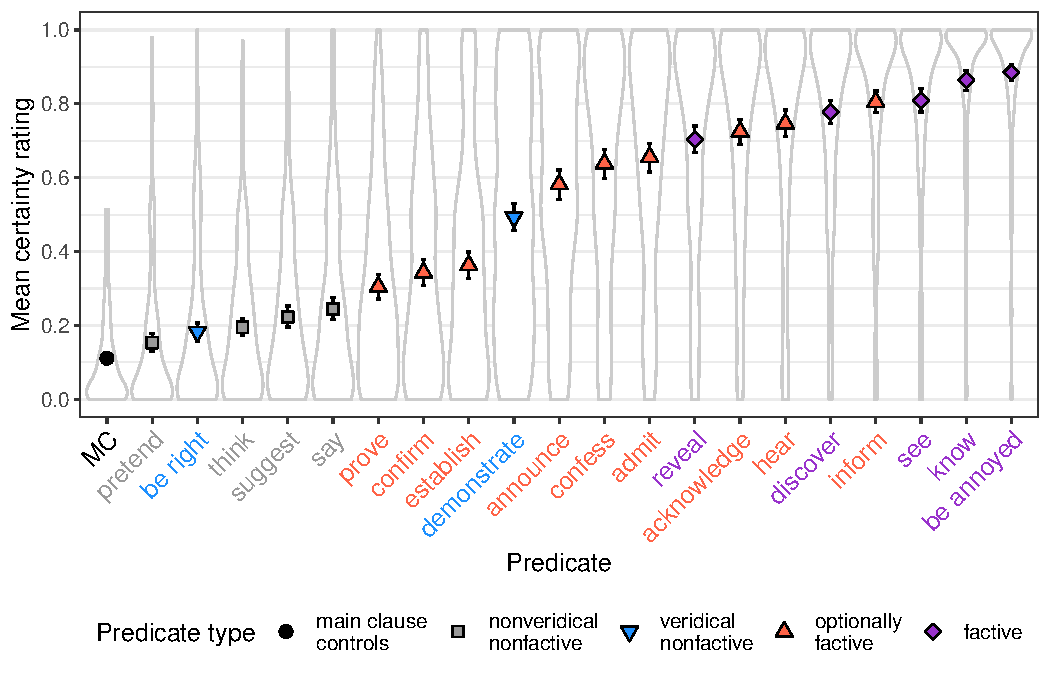
\includegraphics[width=.8\textwidth]{figures/Language-Figure2}
\caption{Mean certainty rating (measuring projection) of main clause content and the CCs of the 20 predicates investigated in Exp.~1a of \citealt{degen-tonhauser-language} (adapted by collapsing the nonfactive predicates into a single category). Error bars indicate 95\% bootstrapped confidence intervals. Violin plots indicate the kernel probability density of the individual participants' ratings.}\label{fig:dt1a}
\end{figure}

Recently,  \citealt[\S6.2]{mandelkern-etal2020} challenged the hypothesis that projection is gradient by arguing that inference rating measures are not suitable to detect binary projection. Such measures are not suitable, they argued, because they do not distinguish between, on the one hand, contents that project because they are presuppositions and, on the other hand, contents that project because they are ``a natural conclusion to draw for any of a variety of pragmatic reasons short of entailment or presupposition'' (p.497). Inference rating measures, they suggested, might invite participants to draw projection inferences even when not lexically required because ``the content in question is right there before the [participants'] eyes" (p.498). They concluded that ``we should think twice before embracing a notion of presupposition projection that is gradient based on results from inference tasks alone'' (p.497).

\citealt[\S6.2]{mandelkern-etal2020} suggested that naturalness ratings of utterances in explicit ignorance contexts are better suited to distinguish presuppositions from nonpresuppositional projection inferences.\footnote{\citealt{mandelkern-etal2020} refer to the measure as an acceptability rating measure, but since participants were asked to rate the naturalness of utterances, we refer to it as a naturalness rating measure.} On this measure, participants are presented with utterances in which a speaker states that they are ignorant about a content, as in (\ref{mtrig}a), and then follows up with an utterance in which the content occurs embedded in an entailment-canceling environment, such as the antecedent of a conditional in (\ref{mtrig}c). \citealt{mandelkern-etal2020} assumed that if the content is a presupposition (such as the pre-state content of {\em stop} in (\ref{mtrig}c)), the utterance is rated as unnatural in the explicit ignorance context because presuppositions are contents that the speaker believes to be true. That is, in such constellations,  participants ``will not have an alternative to interpreting the presupposition at the utterance level, and in turn seeing the utterance as infelicitous and the speaker as incoherent'' (p.497).  If, on the other hand, the content is not a presupposition (such as the pre-state content of {\em now frown on} in (\ref{mtrig}c)), the utterance is assumed to be natural: Even if participants might, in a different context, draw a projection inference ``for any of a variety of pragmatic reasons short of entailment or presupposition, [\ldots] they will tend to relinquish that inclination when there is pragmatic pressure to do so'' as in the explicit ignorance contexts (p.497).\footnote{Presuppositions won't be relinquished, modulo local accommodation} Both presuppositions and nonpresuppositions were expected to be judged as natural in the support contexts, which entail the relevant content, illustrated in (\ref{mtrig}b).

\begin{exe}
\ex\label{mtrig} \citealt[490f.]{mandelkern-etal2020}
\begin{xlist}
\ex Explicit ignorance context: \\ Mary always was involved in a lot of sports, but I don't know whether she ever did any yoga.
\ex Support context: \\ Mary always was involved in a lot of sports, and she used to do yoga, too.
\ex Sentence with presupposition / nonpresupposition: \\ If Mary \{has stopped / now frowns on\} doing yoga, then Matthew will interview her for his story.
\end{xlist}
\end{exe}
\citepos{mandelkern-etal2020} Exp.~3, which used the proposed measure, only provided limited empirical evidence for the hypothesis that projection is a binary property of content. This is primarily because the goal of this work (including Exp.~3) was not to investigate this hypothesis, but rather whether presupposition projection in conjunctions is symmetric. The evidence provided in this work is also limited, however, because only four presupposition triggers and nontriggers each were investigated: The presupposition triggers were the change-of-state verbs {\em stop} and {\em continue}, and the two clause-embedding predicates {\em be aware} and {\em be happy}; the nontriggers were {\em now frown on, enjoy, hope} and {\em be sure}.\footnote{While their Exps.~1 and 2 investigated {\em frown on}, Exp.~3 investigated {\em now frown on}, as shown in (i). It is possible that the pre-state content contributed by this expression is projective: (i), for instance, appears to give rise to the projective content that Mary did not frown on doing yoga in the past. 

\begin{exe}
\exi{(i)} If Mary now frowns on doing yoga, then Matthew will interview her for his story. \hfill (\citealt[491]{mandelkern-etal2020})
\end{exe}
} In the control items of Exp.~3, these eight expressions were realized in (single-clause) antecedents of conditionals, as shown in (\ref{mtrig}c). Naturalness ratings were elicited in explicit ignorance and support contexts. 

\citealt{mandelkern-etal2020} found (as shown in their Fig.~3) that the naturalness ratings for the nontriggers in the control items were relatively high in both contexts (with means just below 5, where 1 meant ``completely unnatural'' and 7 meant ``completely natural'' on their 7-point Likert scale). The presupposition triggers, on the other hand, had lower mean naturalness ratings in the explicit ignorance context (mean around 3) than in the support context (mean just above 5). Mandelkern and his colleagues took this to ``establish[] the effectiveness of the methodology'' (p.492). They proposed (p.497):

\begin{quote}

[\ldots] comparing contexts which support the inference to contexts in which it has been made clear that the speaker is ignorant about the inference provides a way to distinguish a broad class of natural and invited pragmatic inferences from those that are really encoded as presuppositions, and thus have no choice but to project. [...]  In methodological terms, we strongly recommend at least a two-pronged approach, with careful attention paid to results stemming from the evaluation of acceptabilty [sic] in different contexts.

\end{quote}

However, an inspection of the naturalness ratings for the eight (non)triggers provided in Fig.~8 in their Appendix 3 raises doubt about whether the measure indeed provides evidence for a binary distinction between presuppositions and nonpresuppositions. First, considering the mean naturalness ratings in the explicit ignorance contexts, we find ratings for the presuppositions range from just above 1 (for the pre-state of {\em continue}) to about 3.5 (for the CC of {\em be aware}). As the ratings for the nonpresuppositions range from just below 3 (for the CC of {\em hope}) to 4.5 (for the CC of {\em be aware}), it is not clear whether naturalness ratings in explicit ignorance contexts provide evidence for a binary distinction between the four presuppositions and the four nonpresuppositions investigated in \citealt{mandelkern-etal2020}. Second, the effect of context (explicit ignorance vs.\ support) also does not appear to be consistent for presuppositions or nonpresuppositions. Whereas the difference between the mean naturalness ratings in the explicit ignorance and support contexts was quite large for the (presuppositional) pre-state of {\em continue}, the difference was much less pronounced for the (presuppositional) CC of {\em be aware}, where it was roughly comparable to that of the (nonpresuppositional) pre-state of {\em frown on}. In sum, it is not clear that comparisons of ratings in support and explicit ignorance contexts provides empirical support for a binary projection either. 

There also appears to be disagreement in the literature about the naturalness of presuppositions in explicit ignorance contexts. Whereas Mandelkern and his colleagues assumed that all presuppositions are unnatural in explicit ignorance contexts, \citealt{simons01} and \citealt{abusch10} assumed that only hard (nondefeasible) presuppositions are, but that `soft' (defeasible) ones are natural. For instance,  {\em stop} and {\em win} in (\ref{eic2}) were assumed to be natural in explicit ignorance contexts, and {\em again}, the {\em it-}cleft and {\em too} in (\ref{eic3}) unnatural.\footnote{\citealt{abusch10} marked (\ref{eic3}b) and (\ref{eic}c) with `??' instead of `$\#$'.} This disagreement in the literature necessitates further investigation.

\begin{exe}
\ex\label{eic2}
\begin{xlist}
\ex I have no idea whether Jane ever smoked, but she hasn't stopped smoking. \hfill (\citealt[443]{simons01})
\ex I have no idea whether John ended up participating in the
Road Race yesterday. But if he won it, then he has more victories than anyone else in history. \hfill (\citealt[39]{abusch10})
\end{xlist}
\ex\label{eic3}
\begin{xlist}
\ex\infelic I don't know if Jane ever rented ``Manhattan'' before, but perhaps she's renting it again. \hfill (\citealt[443]{simons01})

\ex \infelic I have no idea whether anyone read that letter. But if it is John
who read it, let's ask him to be discreet about the content. \hfill (\citealt[40]{abusch10})

\ex \infelic I have no idea whether John read that proposal. But if Bill read it too, let's ask them to confer and simply give us a yes-no response. \hfill (\citealt[40]{abusch10})
\end{xlist}
\end{exe}

This paper presents the results of an experiment designed to investigate whether the measure proposed by \citealt{mandelkern-etal2020} provides evidence that projection is a binary property of content rather than a gradient one.\footnote{Link to experiment, materials, and analysis scripts: \url{xxx}}  To allow for comparison with the results of \citealt{degen-tonhauser-language}, the CCs of the same 20 (non)factive clause-embedding predicates (see Fig.~\ref{fig:dt1a}) were investigated. The experiment also included control stimuli with {\em stop, continue, again, too, also}, and an {\em it-}cleft, to allow for comparison with the results of \citealt{mandelkern-etal2020} and the assumptions made in \citealt{simons01} and \citealt{abusch10}. 

One change we made to the design of \citepos{mandelkern-etal2020} Exp.~3 was that our experiment implemented a three-level context condition instead of a two-level one. Specifically, we replaced \citepos{mandelkern-etal2020} support context (which entailed the relevant context, see (\ref{mtrig}b)) with two contexts that were compatible with the relevant content but did not entail it. The two contexts differed in the prior probability of the relevant content: In the `lower prior probability' context, illustrated in (\ref{prior}a), the  relevant content (in (\ref{prior}c), that Julian dances salsa) had a comparatively lower prior probability, whereas it had a comparatively higher prior probability in the `higher prior probability' context, illustrated in (\ref{prior}b). These two contexts were normed in \citealt{degen-tonhauser-openmind}. 

\begin{exe}
\ex\label{prior}
\begin{xlist}
\ex Julian is German. \hfill [lower prior probability]
\ex Julian is Cuban. \hfill [higher prior probability]
\ex Did Cole discover that Julian dances salsa?
\end{xlist}
\end{exe}
This change was implemented to allow for comparison to the result of \citealt{degen-tonhauser-openmind}, namely that the projection of a content is sensitive to the content's prior probability. Specifically, this work found that the higher the prior probability of a content, the stronger the projection inference. Under standard analyses of presuppositions, like \citealt{heim83} or \citealt{vds92}, presuppositions are by default globally accommodated in such contexts. Accordingly, such analyses predict that presuppositions are rated as natural in both lower and higher probability contexts, just as in \citepos{mandelkern-etal2020} support contexts. 

%A challenge in the identification of presuppositions is that they only {\em typically} project: It has long been know that presuppositions need not project in any utterance in which the trigging expression is realized (e.g., \citealt{} REFERENCES). For example, in the naturally occurring example in (\ref{acc}) the presupposition of {\em know} (in the framed box) does not project but is (analyzed as) locally accommodated in the scope of the epistemic modal adverb {\em perhaps}. 
%
%
%\begin{exe}
%\ex\label{acc} Whatever the reason, she knows she can't just bounce back, and she decides to leave. For others, the decision is based purely on fear. Perhaps she \fbox{knows} that if she were to stay another day, her life or the lives of her children would be gone. \hfill (\citealt[85]{beaver-belly})
%\end{exe}
%
%
%In view of this potential for presuppositions to not project, investigations into the question of which utterance contents are presuppositions (and which ones are not) must 

\section{Experiment}\label{s2}

To investigate whether the measure proposed in \citealt{mandelkern-etal2020} provides support for a binary distinction between presuppositions and nonpresuppositions, participants read two-sentence discourses consisting of a declarative (which provided the context) and an interrogative (which realized a (non)factive clause-embedding predicate), and rated the naturalness of the interrogative in the context of the declarative.

\subsection{Methods}\label{s-methods}

\subsubsection{Participants}

We recruited 425 participants on Prolific. Due to a server error, the data of only 398 participants was recorded (ages: 19-73, mean: 40.8; 187 women, 201 men, 8 non-binary, 2 preferred to not disclose). The recruited participants were required to live in the USA, to speak English as their first language, to have completed at least 100 tasks, and to have an approval rating of at least 99\%. The median time spent on the task was 6:24 minutes. Participants were paid \$1.78 (corresponding to an hourly pay of \$16.6).


\subsubsection{Materials}

Participants read two-sentence discourses consisting of a declarative followed by an interrogative, as shown in (\ref{sample}). In the target stimuli, the interrogatives combined the 20 (non)factive predicates of \citealt{degen-tonhauser-language} (see Fig.~\ref{fig:dt1a}) with the 20 complement clauses of \citealt{degen-tonhauser-language}, for a total of 400 interrogatives. The preceding declaratives implemented a three-level context condition: In the `explicit ignorance' context (\ref{sample}a), the declarative sentence conveyed the speaker's ignorance about the CC. In the `lower prior probability' context (\ref{sample}b), the CC had a comparatively lower prior probability, whereas it had a comparatively higher prior probability in the `higher prior probability' context (\ref{sample}c). See Supplement \ref{a:clauses} for the full set of 20 complement clauses and the two contexts for each complement clause.

\begin{exe}
\ex\label{sample}
\begin{xlist}
\ex Explicit ignorance context: \\ I have no idea if Julian dances salsa. Does Cole discover that Julian dances salsa?
\ex Lower prior probability context: \\ Julian is German. Did Cole discover that Julian dances salsa?
\ex Higher prior probability context: \\ Julian is Cuban. Did Cole discover that Julian dances salsa?'
\end{xlist}
\end{exe}

In addition to the 1,200 target stimuli (400 interrogatives $\times$ 3 contexts), the materials also included six control stimuli, shown in (\ref{filler}). The interrogatives of the control stimuli featured six expressions typically analyzed as presupposition triggers, namely {\em stop, continue, again, too, also}, and an {\em it-}cleft. The preceding declaratives conveyed the speaker's explicit ignorance about the presuppositions associated with these expressions.\footnote{As the stimuli were presented in writing, prosody was not controlled for. Since the projective contents of {\em too, also}, and the {\em it-}cleft cannot be accommodated, the filler stimuli with these expressions should receive low naturalness in explicit ignorance context under any focus assignment.} Three of these expressions, namely {\em stop, continue,} and {\em again}, were target expressions in the relevant experiments in \citealt{mandelkern-etal2020} and \citealt{kalomoiros-schwarz2021}, who assumed these expressions to be unnatural in explicit ignorance contexts. This is in contrast to \citealt{simons01}, who took {\em stop} to be a soft trigger that is acceptable in explicit ignorance contexts. The other three expressions, namely {\em too, also,} and the {\em it-}cleft, were assumed to be hard triggers in \citealt{simons01} and \citealt{abusch10}, that is, unnatural in explicit ignorance contexts. The control stimuli were included for comparison to the target stimuli, to the claims of \citealt{simons01} and \citealt{abusch10}, and to the results of \citealt{mandelkern-etal2020}.

\begin{exe}
\ex\label{filler} 
\begin{xlist}
\ex I don't know if Stephen was ever in the habit of vaping. Has Stephen recently stopped vaping?
\ex I don't know if John was ever reading ``Dune''. Has John recently continued reading ``Dune''?
\ex I don't know if William was ever interested in history. Is William interested in history again?"
\ex I don't know if Ann plays any instrument. Does Ann play the flute, too?
\ex I don't know if Svenja plays any sport. Does Svenja also play soccer?
\ex I don't know if anyone was playing outside with the kids. Was it Jack who was playing outside with the kids?

\end{xlist}
\end{exe}

The experiment also included 4 filler stimuli that were used to exclude participants not attending to the task (see Supplement \ref{a:fillerPractice}). The filler stimuli were expected to receive high naturalness ratings.

A random set of 30 stimuli was created for each participant. Each set contained 20 target stimuli in which each of the 20 complement clauses was paired with a unique clause-embedding predicate. Twelve of the target stimuli were presented in the explicit ignorance context, and the other eight in a low or a higher prior probability context (four each). Each participants' set of 30 stimuli contained the same six control stimuli and the same four filler stimuli. Each of the 30 stimuli were presented as utterances by a unique named speaker. Trial order was randomized for each participant. 

\subsubsection{Procedure}

Participants were instructed to rate ``how natural the question sounds in the context of the statement''. As shown in Figure \ref{f:trials}, they were asked give their rating on a slider from `totally unnatural' (coded as 0) to `totally natural' (coded as 1). The experiment began with four practice trials to familiarize participants with the task (see Supplement \ref{a:fillerPractice} for details). After responding to the 30 trials, participants filled out a short optional demographic survey. To encourage truthful responses, participants were told that they would be paid no matter what answers they gave in the survey.


\begin{figure}[h]
\centering
%\begin{subfigure}{0.49\textwidth}
\fbox{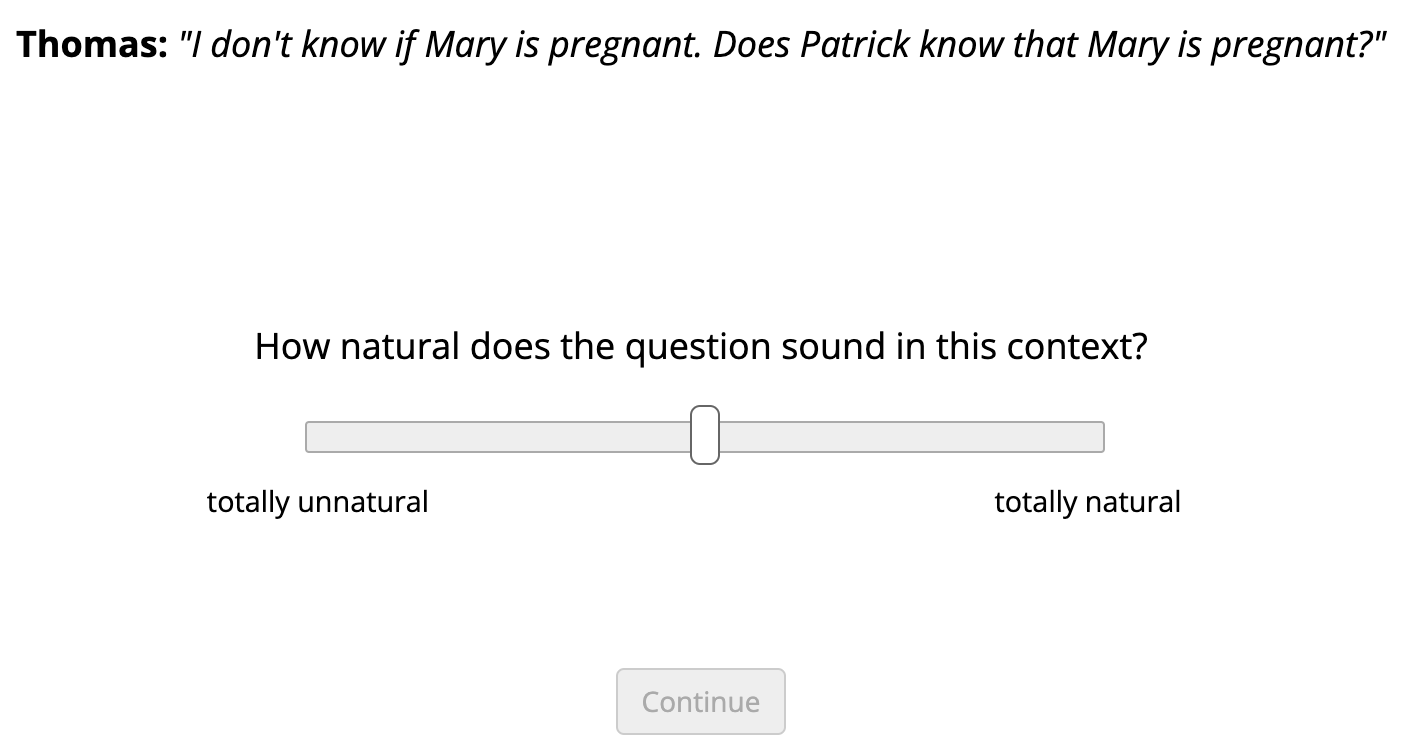
\includegraphics[width=.7\textwidth]{figures/trial-eic}}
%\caption{Trial with explicit ignorance context}
%\end{subfigure}
%\\[.1cm]
%\begin{subfigure}{0.49\textwidth}
%\fbox{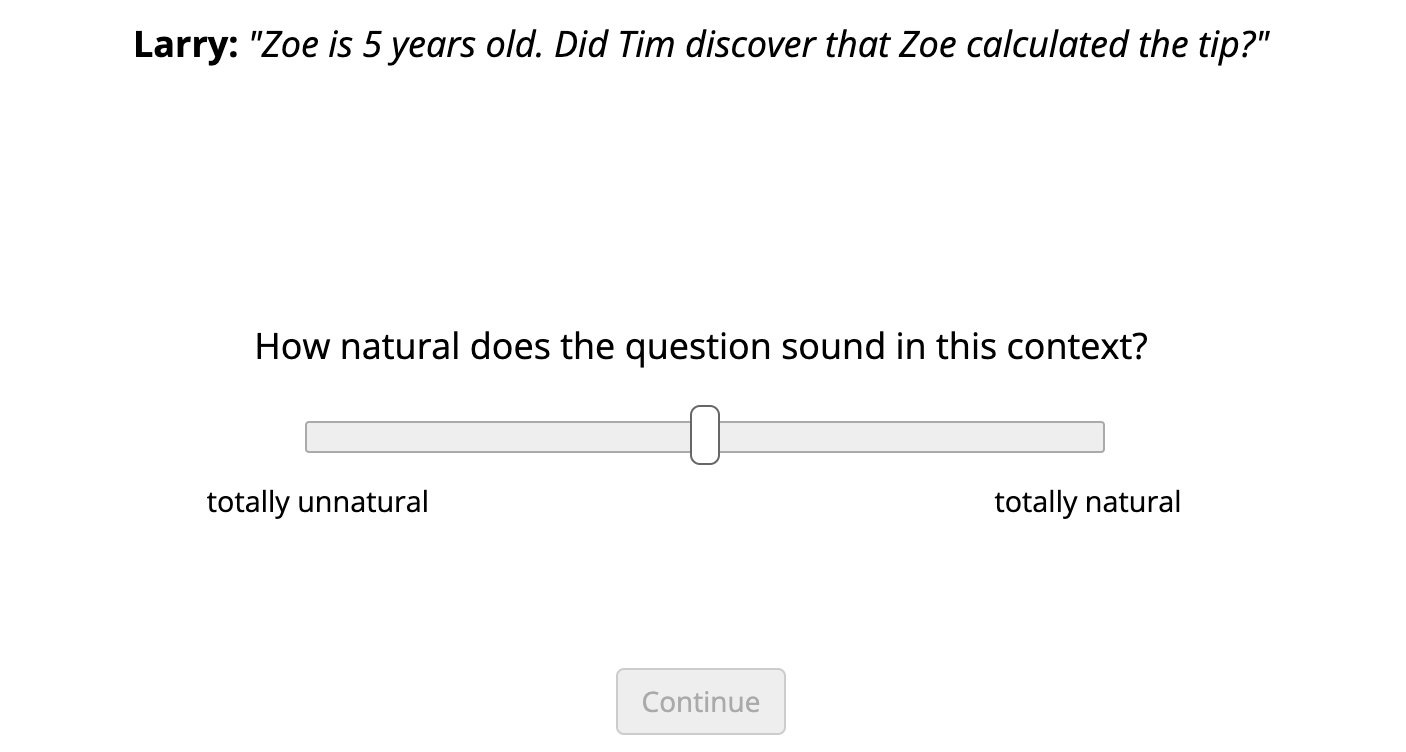
\includegraphics[width=\textwidth]{figures/trial-low}}
%\caption{Trial with lower prior probability context}
%\end{subfigure} \hfill \begin{subfigure}{0.49\textwidth}
%\fbox{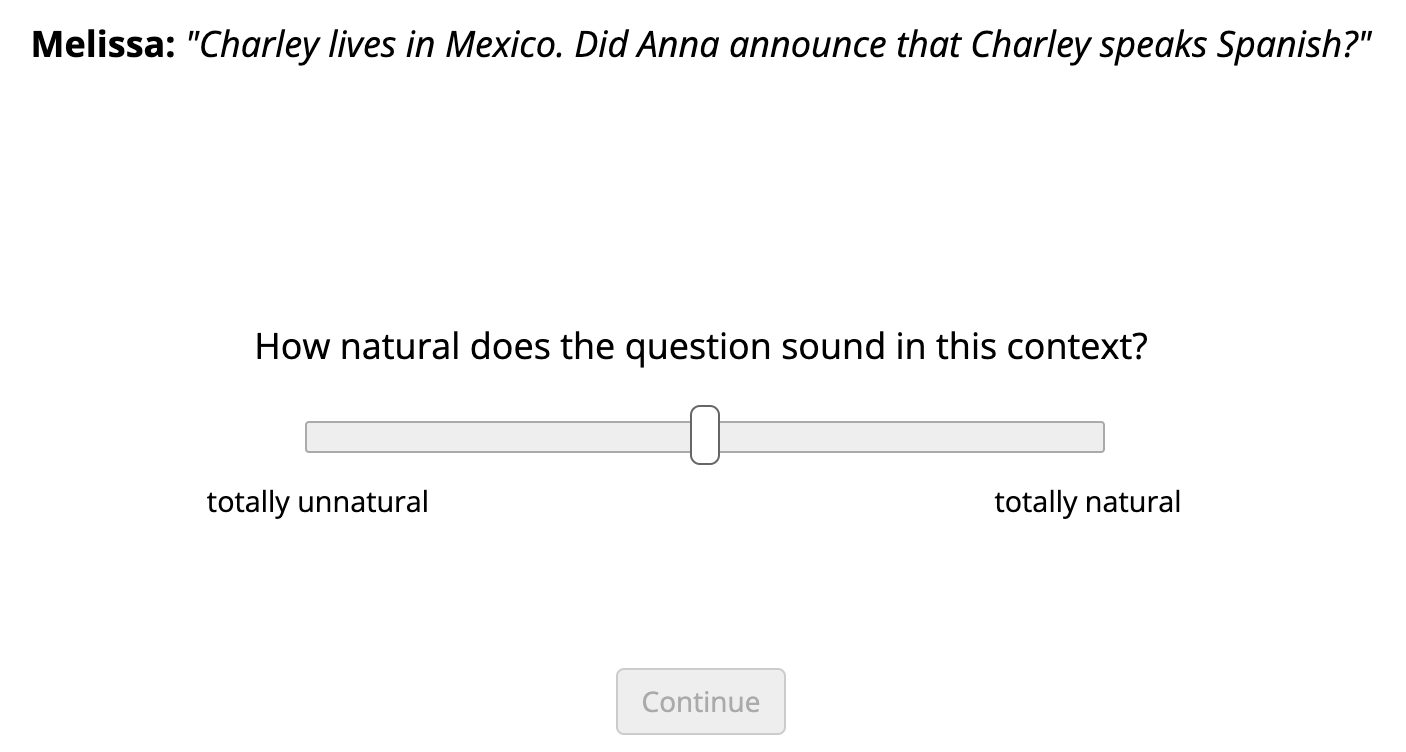
\includegraphics[width=\textwidth]{figures/trial-high}}
%\caption{Trial with higher prior probability context}
%\end{subfigure}
\caption{Sample experiment trial with explicit ignorance context.}\label{f:trials}
\end{figure}


\subsubsection{Data exclusion} 

We excluded the data of five participants who did not self-identify as native speakers of American English as well as the data of 23 participants whose mean response to the attention checks was more than 2 sd below the group mean.\footnote{Contrary to what was preregistered, one of the four controls was not used to exclude participants because it received a mean rating of only .5. See Supplement \ref{a:fillerPractice} for details.} The data of 370 participants entered into the analysis (ages: 19-80, mean: 40.7; 175 women, 185 male, 8 non-binary, 2 preferred to not disclose). Each of the 20 predicates received at least 200 ratings in the explicit ignorance context (mean: 222 ratings), at least 59 ratings in the lower prior probability context (mean: 74), and at least 61 ratings in the higher prior probability context (mean: 74). The six control stimuli received 370 ratings each. 

\subsection{Results}

We first address the question of whether naturalness ratings in explicit ignorance contexts provide empirical evidence for a binary difference between presuppositions and nonpresuppositions (\S\ref{s:analysis1}). We then consider whether a comparison of naturalness ratings in the contexts provides such evidence (\S\ref{s:analysis2}).

\subsubsection{Naturalness ratings in explicit ignorance contexts}\label{s:analysis1}

Recall that \citealt{simons01} and \citealt{abusch10} assumed that hard presuppositions are unnatural in explicit ignorance contexts, whereas \citealt{mandelkern-etal2020} assumed that all presuppositions are unnatural in such contexts. Figure \ref{fig:acc-by-expression} shows the mean naturalness ratings in the explicit ignorance context by expression (in distinct colors: \color{orange}factive predicates\color{black}, \color{green}nonfactive predicates\color{black},  controls). As shown, purported presuppositions, that is, the controls and the factive predicates, do not exhibit a unified pattern: The mean naturalness ratings of four controls ({\em continue, too, also, again}) is at floor, those of {\em stop} and {\em be annoyed} are a bit higher, those of the {\em it-}cleft and {\em know} are higher again,\footnote{The distribution of the ratings for the CC of {\em know} is bimodal. We discuss this in \S\ref{s3}.} and those of {\em see, discover}, and {\em reveal} are just as high as the means of some nonfactive predicates. These results do not provide empirical support for a binary distinction between presuppositions and nonpresuppositions, contrary to what \citealt{mandelkern-etal2020} hypothesized. Furthermore, these results do not provide empirical support for for a class of factive predicates that is categorically distinct from nonfactive predicates, in line with the result of \citealt{degen-tonhauser-language} based on inference rating measures. 

\begin{figure}[h!]
\centering
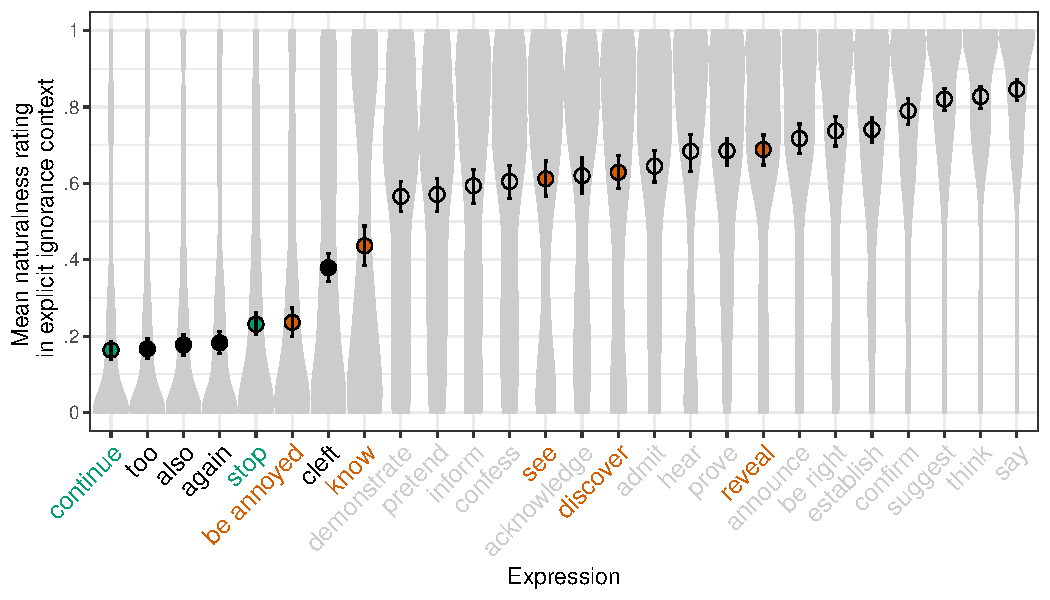
\includegraphics[width=1\textwidth]{../../results/main/13explicitIgnorance/graphs/explicit-ignorance-naturalness-by-predicate}
\caption{Mean naturalness rating in explicit ignorance context by expression (\color{orange}factive\color{black}, \color{green}nonfactive\color{green}, \color{black}filler\color{black}). Error bars indicate 95\% bootstrapped confidence intervals. Overlaid violin plots indicate the kernel probability density of the participants' ratings.}\label{fig:acc-by-expression}
\end{figure}

These observations were confirmed by a posthoc pairwise comparison of the naturalness ratings of the contents associated with the six controls and 20 target expressions using the `emmeans' package (\citealt{emmeans}) in R (\citealt{r}). The input to the pairwise comparison came from a Bayesian mixed-effects beta regression model with weakly informative priors using the `brms' package (\citealt{buerkner2017}). The model predicted naturalness ratings from a fixed effect of expression (with treatment coding and `continue' as reference level) and included random by-participant and by-item intercepts (where an item is a complement clause). We thus obtain, for each predicate, a 95\% credible interval for the mean rating for that predicate. This analysis provided us with with posterior distributions of estimated marginal means of pairwise differences. We assume that two expressions differ in their mean naturalness rating when the posterior distribution of their difference does not include 0. See Supplement \ref{a:analysis1} for the full model output. 

As shown in Table \ref{t:pairwise}, the analysis suggests difference between the naturalness ratings of the factive predicates in the explicit ignorance context: the ratings of {\em be annoyed} are lower than those of {\em know}, which in turn are lower than those of {\em see} and {\em discover}, which in turn are lower than those of {\em reveal}. Furthermore, the naturalness ratings for the CCs of the five factive predicates are indistinguishable from different sets of expressions: The naturalness ratings for {\em be annoyed} do not differ from those of {\em stop} (but are higher than those the prejacents of the controls {\em continue, too}, and {\em also}), the naturalness ratings for {\em know} do not differ from those of the {\em it-}cleft, the naturalness ratings for {\em see} and {\em discover} do not differ from those of the nonfactives {\em confess, acknowledge}, and {\em admit}, and those of {\em reveal} do not differ from those of the nonfactives {\em prove} and {\em announce}. These results confirm that naturalness ratings in explicit ignorance contexts do not provide empirical support for a binary distinction between factive and nonfactive predicates, or between presuppositions and nonpresuppositions.

\begin{table}[!h]
\begin{center}
\begin{tabular}{r ccccccccccccccccccccccccc}
\toprule
 &  \rot{continue} & \rot{too} & \rot{also} & \rot{again} & \rot{stop} & \rot{be annoyed} & \rot{cleft} & \rot{know} & \rot{demonstrate} & \rot{pretend} & \rot{inform} & \rot{confess} & \rot{see} & \rot{acknowledge} & \rot{discover} & \rot{admit} & \rot{hear} & \rot{prove} & \rot{reveal} & \rot{announce} & \rot{be right} & \rot{establish} & \rot{confirm} & \rot{suggest} & \rot{think} \\
 \midrule
 too & & & & & & & & & & & & & & & & & & \\
also & & & & & & & & & & & & & & & & & & \\
again  & & & & & & & & & & & & & & & & & & \\
stop  & & & & & & & & & & & & & & & & & & \\
be annoyed & & & & & & & & & & & & & & & & & & \\
cleft & & & & & & & & & & & & & & & & & & \\
know & & & & & & & & & & & & & & & & & & \\
demonstrate & & & & & & & & & & & & & & & & & & \\
pretend & & & & & & & & & & & & & & & & & & \\
inform & & & & & & & & & & & & & & & & & & \\
confess & & & & & & & & & & & & & & & & & & \\
see & & & & & & & & & & & & & & & & & & \\
acknowledge & & & & & & & & & & & & & & & & & & \\
discover & & & & & & & & & & & & & & & & & & \\
admit & & & & & & & & & & & & & & & & & & \\
hear & & & & & & & & & & & & & & & & & & \\
prove & & & & & & & & & & & & & & & & & & \\
reveal & & & & & & & & & & & & & & & & & & \\
announce & & & & & & & & & & & & & & & & & & \\
be right & & & & & & & & & & & & & & & & & & \\
establish & & & & & & & & & & & & & & & & & & \\
confirm & & & & & & & & & & & & & & & & & & \\
suggest & & & & & & & & & & & & & & & & & & \\
say  & & & & & & & & & & & & & & & & & & \\
\bottomrule
\end{tabular}
\caption{Posterior distributions of estimated marginal means of pairwise differences `***' indicates significance at .001, `**' at .01, `*' at .05, `.' marginal significance at .1, and \emph{n.s} indicates no significant difference in means.}\label{t:pairwise}
\end{center}
\end{table}

Contrary to what is assumed in \citealt{mandelkern-etal2020} and \citealt{kalomoiros-schwarz2021}, presuppositions are not invariably unnatural in explicit ignorance contexts. Rather, in line with what was assumed in \citealt{simons01} and \citealt{abusch10}, some presuppositions seem to be rated as more unnatural in such contexts than others. On the assumption that naturalness ratings in explicit ignorance contexts differentiate between undefeasible/hard and defeasible/soft triggers, one might take the results of our experiment to suggest that the pre-state contents of {\em continue} and {\em again}, and the existence requirements of {\em too} and {\em also} are not defeasible. The CCs of {\em see, discover}, and {\em reveal}, on the other hand, might be taken to be defeasible. Contrary to what \citealt{abusch10} assumed, the existence requirement of the {\em it-}cleft is not as clearly undefeasible as that of other projective contents (\citealt{smith-hall11} also observed that the {\em it-}cleft did not pattern like a hard trigger in their experiment.) The results of our experiment align with our observation about possible by-content variation in \citepos{mandelkern-etal2020} Exp.~3. Recall from above that in their Exp.~3, the pre-state of {\em continue} was judged as (numerically) less natural in explicit ignorance contexts than the CC of the cognitive predicate {\em be aware}. This result is in line with the result of our experiment that the pre-state of {\em continue} is judged as less natural than the CC of the cognitive predicate {\em know}.

\subsubsection{Comparison of naturalness ratings across contexts}\label{s:analysis2}

We next consider whether presuppositions and nonpresuppositions differ with respect to the ratings in contexts in which the speaker is explicitly ignorant of the content and in contexts that are compatible with the content. Recall that \citealt{mandelkern-etal2020} expected presuppositions to be sensitive to their context manipulation (explicit ignorance vs.\ support) but not nonpresuppositions. Fig.~\ref{fig:acc-by-context} shows mean naturalness ratings for the CCs of the 20 \fcolorbox{black}{orange}{factive} and \fcolorbox{black}{green}{nonfactive} predicates in the three contexts featured in our experiment, with the predicates ordered by their mean naturalness ratings in the explicit ignorance context, as in Fig.~\ref{fig:acc-by-expression}. 

As shown, the effect of context is not uniform for the factive predicates: For {\em be annoyed} and {\em know}, the mean naturalness rating is lower in the explicit ignorance context than in the higher prior probability context, the two ratings are equally high for {\em see, discover}, and {\em reveal}. This latter pattern is also observed for many of the nonfactive predicates, for instance {\em confess, hear, announce}, and {\em be right}. Thus, naturalness ratings in explicit ignorance vs.\ higher prior probability contexts do not provide support for a binary distinction between the CCs of factive and nonfactive predicates. A comparison between the explicit ignorance and lower prior probability contexts also suggests variation between the factive predicates: Whereas for {\em be annoyed} the mean naturalness ratings are lower in the explicit ignorance context than in the lower prior probability context, they are equally high for {\em know}, but lower in the lower prior probability context than the explicit ignorance context for {\em see, discover}, and {\em reveal}. This latter pattern is observed for all of the nonfactive predicates, except possibly {\em pretend}. Thus, naturalness ratings in explicit ignorance vs.\ lower prior probability contexts also do not provide support for a binary distinction between the CCs of factive and nonfactive predicates. 

Finally, we observe that the prior probability of content modulates its naturalness ratings for all predicates, except {\em demonstrate} and {\em pretend}): Content is judged as more natural in a context in which it has a higher prior probability than in a context in which it has a lower prior probability. This result is in line with the result of \citealt{degen-tonhauser-openmind} based on an inference rating task.

\begin{figure}[h!]
\centering
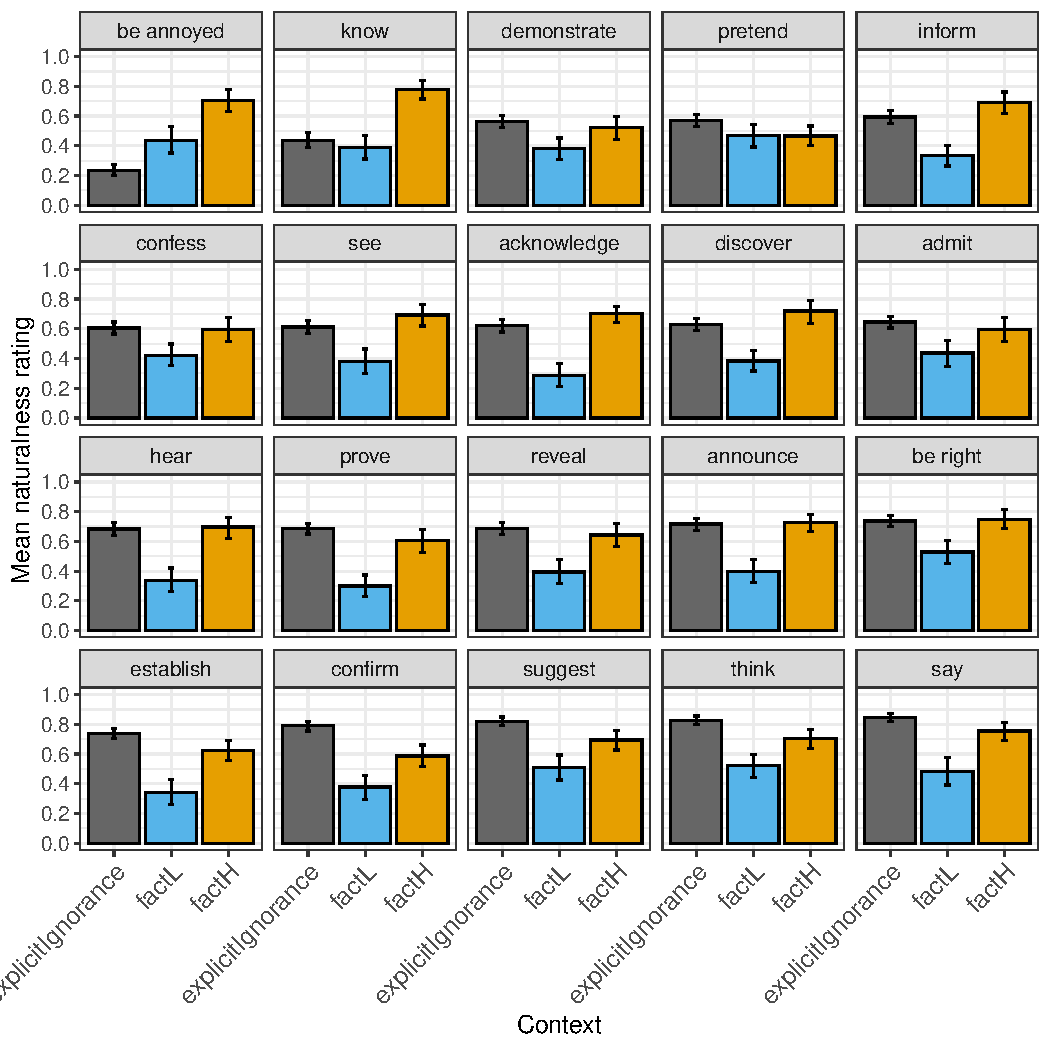
\includegraphics[width=\textwidth]{../../results/main/13explicitIgnorance/graphs/naturalness-by-context-and-predicate}
\caption{\small{Mean naturalness rating by context and predicate (\fcolorbox{black}{orange}{factive}, \fcolorbox{black}{green}{nonfactive}); predicates ordered as in Fig.~\ref{fig:acc-by-expression}. Error bars indicate 95\% bootstrapped CIs. Violin plots indicate kernel probability density of participants' ratings}.}\label{fig:acc-by-context}
\end{figure}

These results were confirmed by a model...{\bf BETA MODELS}

\newpage

bla

\newpage

\section{Discussion}\label{s3}

The experiment was designed to investigate \citepos{mandelkern-etal2020} claim that the measure used in their Exp.~3 provides empirical support for the hypothesis that projection is a binary property of content and distinguishes presuppositions from nonpresuppositions. Neither the by-content comparison of naturalness ratings in explicit ignorance contexts nor the by-context comparison of naturalness ratings provided empirical support for a binary distinction between the CCs of factive and nonfactive predicates, or, more generally, between presuppositions and nonpresuppositions. In sum, the experiment did not find support for \citepos{mandelkern-etal2020} claim nor for the hypothesis that projection is a binary property of content. Instead, the experiment provided further support for the hypothesis of \citealt{tbd-variability} that projection is a gradient property of content and the result of \citealt{degen-tonhauser-language} that there is no well-defined class of factive predicates. In this section, we discuss theoretical and methodological implications of these results.

\subsection{What are presuppositions?}

Contemporary literature still frequently treats presuppositions as if they were a homogenous class, for instance by characterizing them as contents that typically project or as felicity requirements. Research on projective content has long recognized that the set of contents that have been called presuppositions is heterogeneous. Two dimensions of variation that were already mentioned in \S\ref{s1}, namely defeasibility and strength of projection, fly in the face of this homogeneity assumption.  A third dimension of variation is whether the presupposition is associated with what \citealt{brst-lang11} referred to as a `strong contextual felicity' constraint: Some presumed presuppositions are not associated with such a constraint, which means that they are judged to be acceptable in a context that is neutral with respect to the content (like the CC of {\em know}, which is informative in such a context), while others are associated with such a constraint, that is, judged to be unacceptable in a context that does not entail or satisfy the content (like the existence requirement of pronouns or {\em too}). A fourth dimension of variation is at-issue, that is, whether the content can address the Question Under Discussion: As shown in \citealt{tbd-variability}, the CCs of factive predicates vary in this regard, as the CC of {\em discover} is more at-issue than those of  {\em be annoyed} and {\em know}.

Given that the set of contents called presuppositions is heterogeneous, it is not entirely surprising that these contents do not pattern alike in explicit ignorance contexts. For instance, a content that is associated with a strong contextual felicity constraint, like the existence requirement of {\em too}, might be expected to be judged as unnatural in a context in which the speaker is explicitly ignorant about the content. On the other hand, a content that is not associated with a strong contextual felicity constraint and that can be at-issue, like the CC of {\em discover}, might be expected to be judged as somewhat natural in a context in which the speaker is explicitly ignorant about the content, as the content can be interpreted as what the speaker is inquiring about. Our experiment suggests that both of these expectations were borne out by the data. 

\begin{exe}
\ex
\begin{xlist}
\ex If Julian dances salsa, then Cole knows that he does.
\ex If Julian dances salsa, then 
\end{xlist}
\end{exe}

Against this background, it does not seem fruitful to us to 

\begin{itemize}

\item When \citealt{mandelkern-etal2020} talk about presuppositions, it's not even clear what they mean: +SCF or -SCF? They only investigated -SCF/+OLE expression but assumed an analysis for them that was developed for +SCF triggers.

\end{itemize}

{\bf need to discuss in the results what naturalness in EIC appears to be sensitive to, and also bimodal for know and low responses for be annoyed}

\subsection{Is projection a binary or a gradient property of content?}

\begin{itemize}

\item We need to identify which level we're talking about

\begin{itemize}

\item Speaker belief:

Option 1: Speaker belief is binary, gradience is introduced by interpretation.

Option 2: Speaker belief is gradient.

\item Lexical representation:

Option 1: Representation codes projection

Option 2: Representation does not code projection but projection is possible in particular utterances

\end{itemize}

\item Typically, researchers ask this because they wonder about the linguistic representation we want to assume in our models. Simple picture:

triggers introduce context requirement and hence content typically projects

nontriggers do not introduce this and hence exhibit projection to varying degrees

\item More complex picture, already represented by contemporary analyses:

+SCF: introduce anaphoric requirement/felicity requirement

soft triggers: lexical meaning typically gives rise to projection inference

nontriggers: lexical meaning may give rise to projection inference

\item To address this question, we have to distinguish whether we're talking about content associated with a particular expression (aggregated projection over multiple utterances) versus utterance content

\item The characterization of presuppositions is at the level of content, but has to involve `typically' to capture that a presupposition in some utterances does not project.

\item We also have to distinguish the speaker and the hearer: The speaker may be binary or gradient, and even if binary, interpretation may vary because of different assumptions about speaker, different integration of other factors.

\item Projection inferences, sources of gradience

\begin{tabular}{l c c c c} \\ 
             & expression & utterance & speaker & interpreter \\\hline
class 1 &  binary & binary & binary & binary \\
class 2 &  binary & & & \\ 
class 3 & & & & \\

\end{tabular}


\item What does gradient projection mean?

\begin{itemize}

\item[{[H1]}] Projection is binary at the level of the expression: An expression either triggers a presupposition or not. The observed gradience at the utterance level is due to utterance-level factors that modulate projection.

\item[{[H2]}] Projection is not binary at the level of the expression: The lexical representations of (classes of) expressions give rise to projection inferences of varying strength. The observed gradience at the utterance level is due to the lexical variation in projection strength as well as utterance-level factors that modulate projection.

\end{itemize}

\item Contemporary presupposition analyses (e.g., \citealt{heim83,vds92,abrusan2011,karttunen2016,simons-etal2017}) predict neither the heterogeneity of the naturalness ratings of factive predicates nor their sensitivity to the prior probability of the CC (though see \citealt{schlenker2021} for the latter). These results, which mirror those based on inference ratings, suggest that projection analyses must incorporate more fine-grained distinctions between attitude predicates and the systematic effect of prior probabilities on projection.

\end{itemize}

\subsection{Which measures are suitable to investigate projection?}



\begin{itemize}

\item And while naturalness ratings in EICs may provide insight into the meanings of attitude predicates, the interpretation of the results depends on the presumed linking function (see, e.g., \citealt{sprouse2018}). Instead of the ratings directly reflecting whether the CC is presupposed, the very low mean rating for {\em be annoyed} in EICs could be due to its CC being not-at-issue while the EIC suggests that it is at-issue; likewise, reading {\em know} with a contrastive pitch accent in EICs may have resulted in about half of the participants giving a high rating.


\item This result suggests that interrogatives are particularly acceptable when the speaker is either ignorant about the CC or the CC has a higher prior probability: to inquire about the CC, or to inquire about the matrix clause. 

\item We also observe that the mean naturalness rating is lower in the lower prior probability context than in the higher prior probability context, for all of the predicates except for {\em pretend}. This suggests that the prior probability of the CC modulates the naturalness of the interrogative regardless of whether the embedding predicate is factive, where the observed context-sensitivity is unexpected under standard analyses (e.g., \citealt{heim83,vds92}) or nonfactive (where it is expected). This result mirrors that of \citealt{degen-tonhauser-openmind}, who found in an inference rating task the strength of projection inferences to the CCs of factive and nonfactive predicates is modulated by the prior probability of the CC. One could, of course, propose to make the global accommodation of presuppositions to not be default but to be sensitive to the prior probability of content. But the fact of the matter is that the context-sensitivity is observed not just for factive but also for nonfactive predicates, thereby motivating a common projection mechanism.

\item The talk also discusses that the results do not align with assumptions about hard and soft triggers; \citealt{simons01,abusch10}.

\end{itemize}

\subsection{What does an empirically adequate analysis of projection need to capture?}

\section{Conclusions}\label{s4}

% end document here for word count
%\end{document}

\bibliographystyle{../cslipubs-natbib}
%\bibliographystyle{/Users/tonhauser.1/Library/Latex/cslipubs-natbib}
\bibliography{/Users/tonhauser.1/Documents/bibliography}

\newpage

\section*{Supplemental materials}

\appendix

\setcounter{page}{1}
%\renewcommand{\thetable}{A\arabic{table}}

\setcounter{table}{0}
\renewcommand{\thetable}{A\arabic{table}}

\setcounter{figure}{0}
\renewcommand{\thefigure}{A\arabic{figure}}

\section{Experiment stimuli}\label{a:clauses}

The twenty predicates used in the experiment are the same as in \citealt{degen-tonhauser-openmind,degen-tonhauser-language}:

\begin{exe}
\ex\label{predicates}
\begin{xlist}
\ex Factive: be annoyed, discover, know, reveal, see
\ex Non-factive: acknowledge, admit, announce, be right, confess, confirm, establish, hear, inform, pretend, prove, say, suggest, think
\end{xlist}
\end{exe}

Eventive predicates, like {\em discover} and {\em hear}, were realized in the past tense and stative predicates, like {\em know} and {\em be annoyed}, were realized in the present tense. The direct object of {\em inform} was realized by the proper name {\em Sam}. Each clause-embedding predicate was paired with a unique subject proper name. The speaker of the target stimuli was realized by a randomly sampled unique proper name. 

The following list shows the 20 clauses that realized the complements of the predicates in the target and filler stimuli, together with their lower and higher probability facts, respectively, that realized the preceding declarative sentences in the filler stimuli.

\begin{enumerate}[leftmargin=4ex,itemsep=-2pt]
\item Mary is pregnant. Facts: Mary is a middle school student / Mary is taking a prenatal yoga class
\item Josie went on vacation to France. Facts:  Josie doesn't have a passport / Josie loves France 
\item Emma studied on Saturday morning. Facts: Emma is in first grade / Emma is in law school 
\item Olivia sleeps until noon. Facts: Olivia has two small children / Olivia works the third shift
\item Sophia got a tattoo. Facts: Sophia is a high end fashion model / Sophia is a hipster
\item Mia drank 2 cocktails last night. Facts: Mia is a nun / Mia is a college student
\item Isabella ate a steak on Sunday. Facts: Isabella is a vegetarian / Isabella is from Argentina
\item Emily bought a car yesterday. Facts: Emily never has any money / Emily has been saving for a year
\item Grace visited her sister. Facts: Grace hates her sister / Grace loves her sister
\item Zoe calculated the tip. Facts: Zoe is 5 years old / Zoe is a math major
\item Danny ate the last cupcake. Facts: Danny is a diabetic / Danny loves cake
\item Frank got a cat. Facts: Frank is allergic to cats / Frank has always wanted a pet
\item Jackson ran 10 miles. Facts: Jackson is obese / Jackson is training for a marathon
\item Jayden rented a car. Facts: Jayden doesn't have a driver's license / Jayden's car is in the shop
\item Tony had a drink last night. Facts: Tony has been sober for 20 years / Tony really likes to party with his friends
\item Josh learned to ride a bike yesterday. Facts: Josh is a 75-year old man / Josh is a 5-year old boy
\item Owen shoveled snow last winter. Facts: Owen lives in New Orleans / Owen lives in Chicago
\item Julian dances salsa. Facts: Julian is German / Julian is Cuban
\item Jon walks to work. Facts: Jon lives 10 miles away from work / Jon lives 2 blocks away from work
\item Charley speaks Spanish. Facts: Charley lives in Korea / Charley lives in Mexico
\end{enumerate}

\section{Control and practice stimuli}\label{a:fillerPractice}

The following list shows the four control stimuli where the interrogative was expected to receive high naturalness ratings in the context of the preceding declarative sentence. The values in parentheses indicate the mean naturalness rating for each of the four controls. As shown, the third control did not receive the expected high naturalness mean ratings (probably because participants were unwilling to accommodate that Hendrick has a car in a context in which Hendrick was looking to buy a car). This control was therefore not used to exclude participants' data. 

\begin{enumerate}[leftmargin=4ex,itemsep=-2pt]

\item I don't know if Samantha has a new hat. Does Samantha have a new hat? (.89)

\item  I don't know if this pizza has mushrooms on it. Does this pizza have mushrooms on it? (.87)

\item Hendrick was looking to buy a car. Was Hendrick's car expensive? (.5)

\item Mary visited her aunt yesterday. Is Mary's aunt sick? (.91)

\end{enumerate}

\noindent
The following list shows the four practice stimuli in the order in which they were presented to the participants. Participants were able to advance to the experiment only if they gave a naturalness rating higher than .6 for the first and third stimulus, and a naturalness rating lower than .4 for the second and fourth stimulus.

\begin{enumerate}[leftmargin=4ex,itemsep=-2pt]

\item I have no idea where Natalie is from. Is Natalie from the USA?

\item I don't have any sisters. Have you met my sister yet?

\item I am going on vacation to Ireland. Does Fritz realize that Joe is going with me?

\item I have no idea if Anna has any dogs. Is Samuel glad that Anna fed her dogs?

\end{enumerate}

\section{Model output: Pairwise comparison of expressions}\label{a:analysis1}

\begin{sidewaysfigure}[h!]
\centering
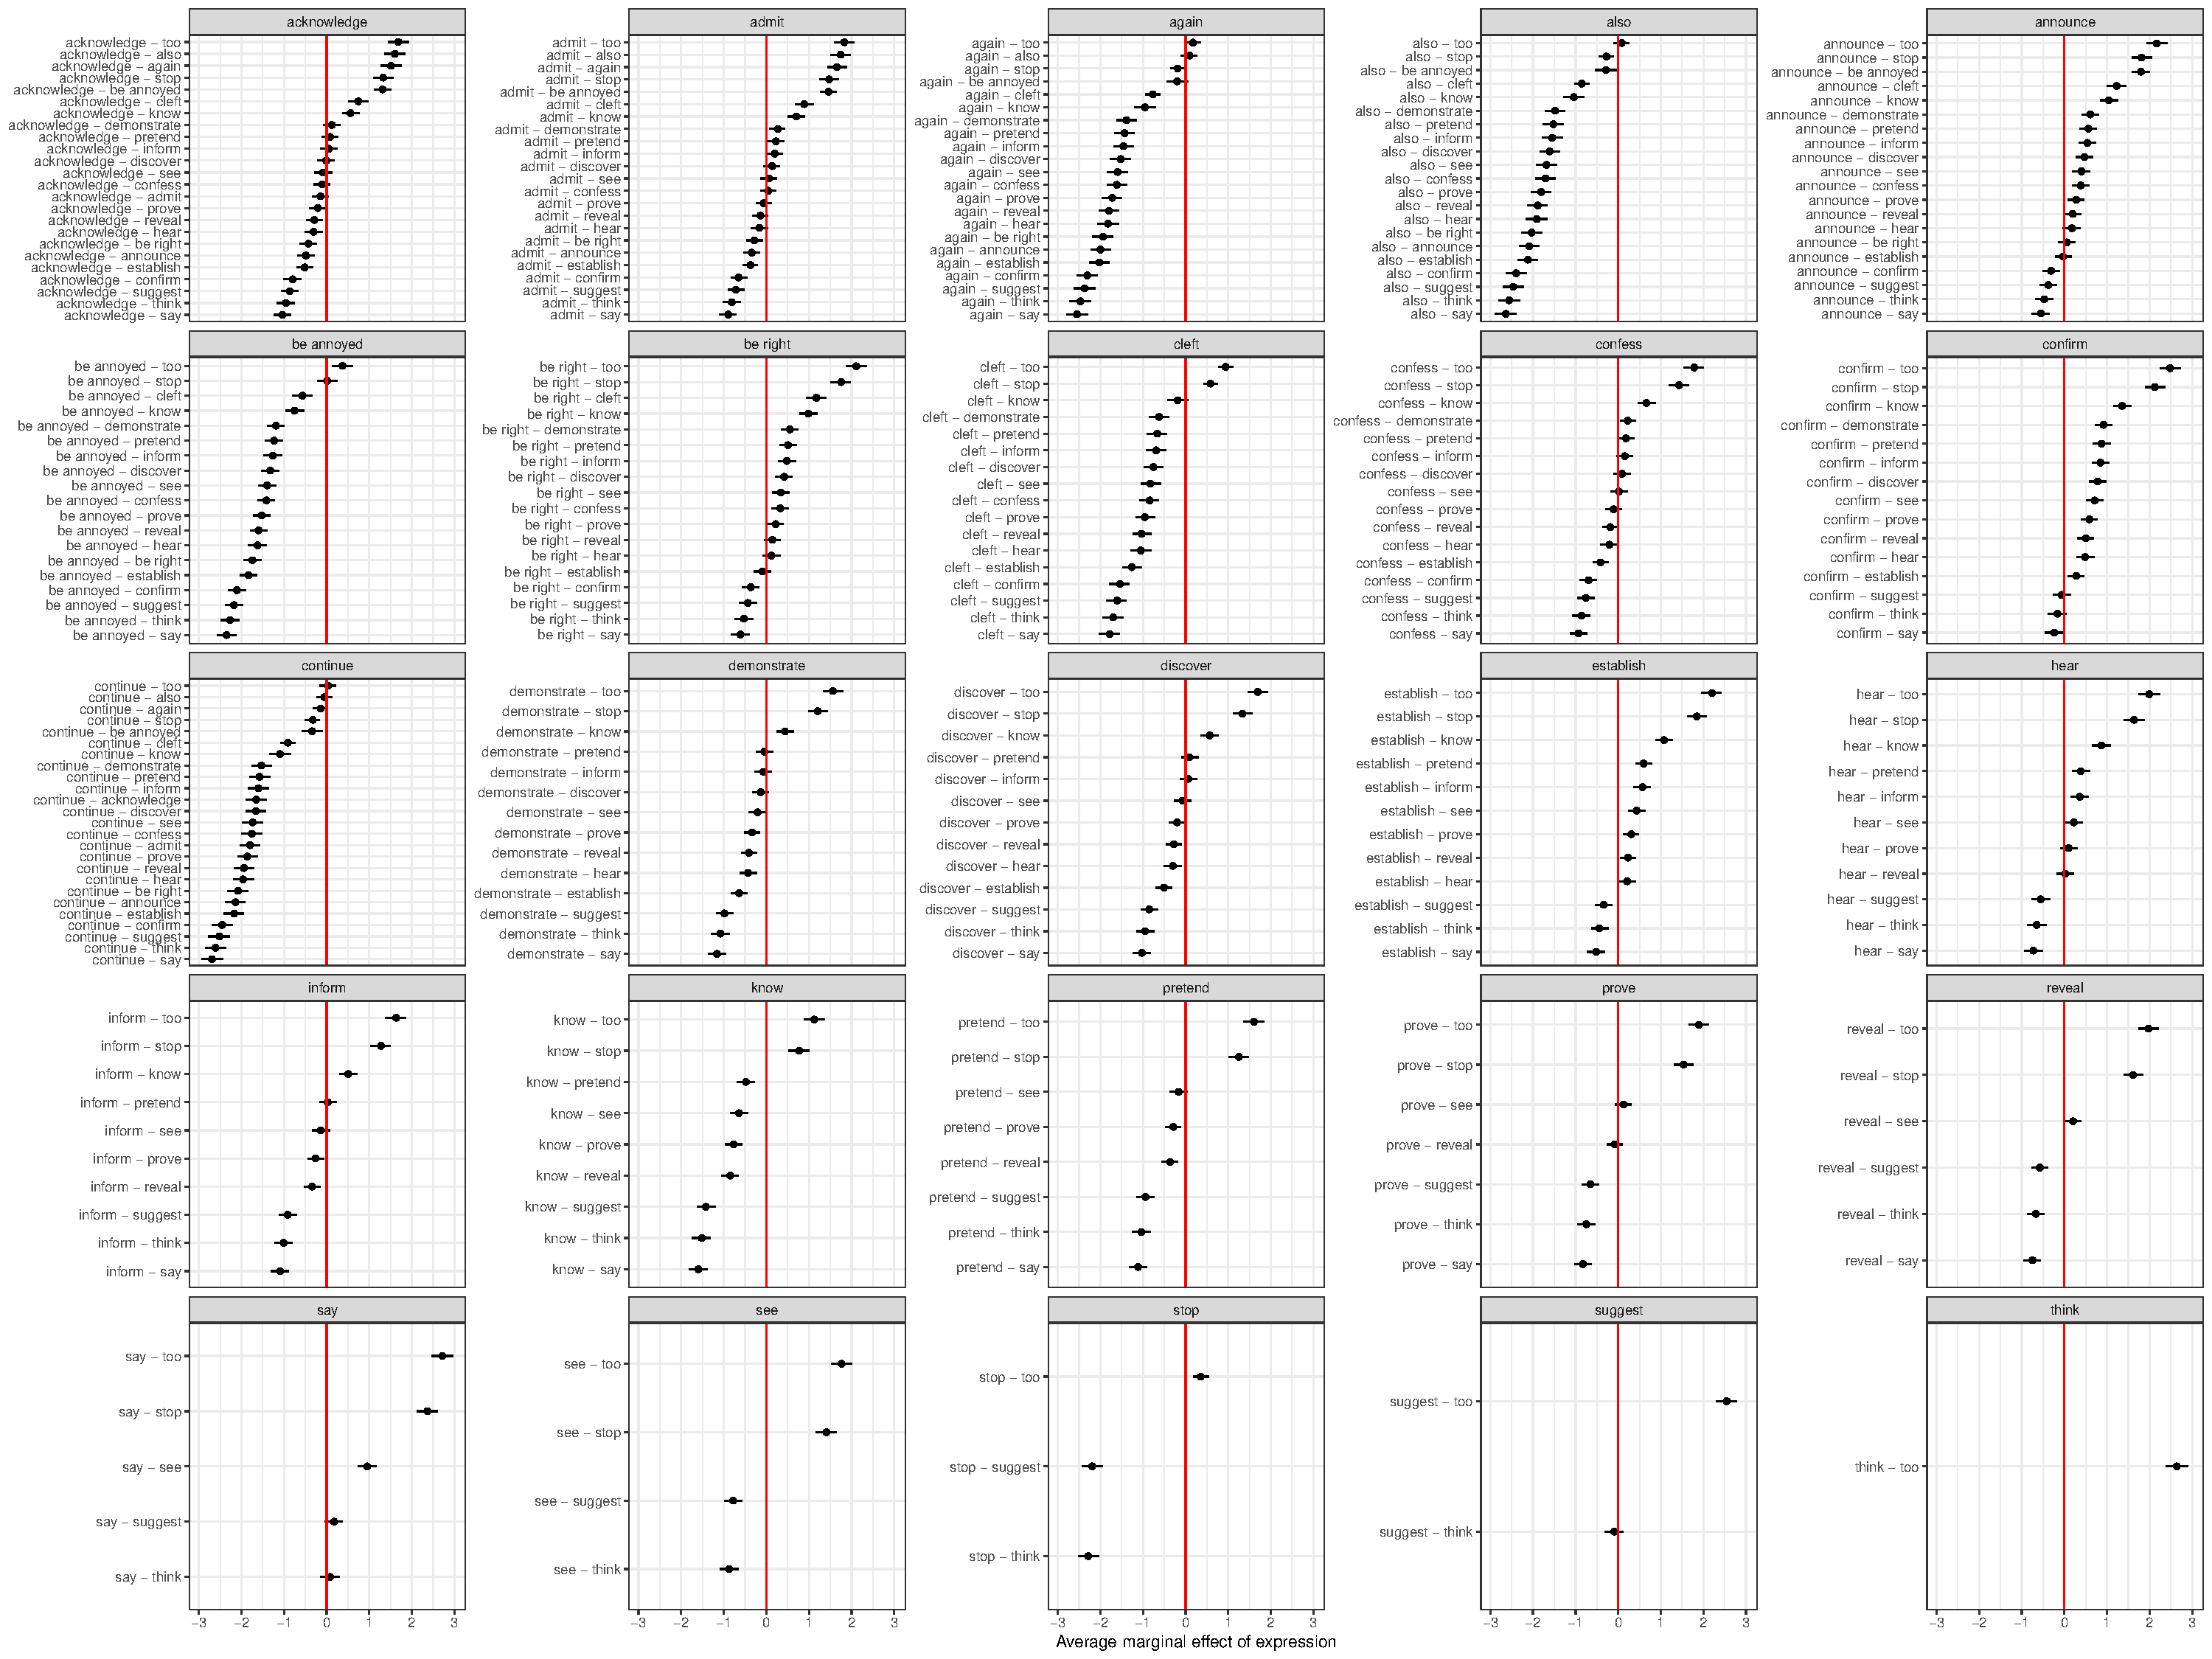
\includegraphics[width=\textwidth]{../../results/main/13explicitIgnorance/graphs/comparisons-in-EIC}
\caption{.}\label{fig:comparisons1}
\end{sidewaysfigure}

\section{Model output: Pairwise comparison of contexts}\label{a:analysis2}

\begin{figure}[h!]
\centering
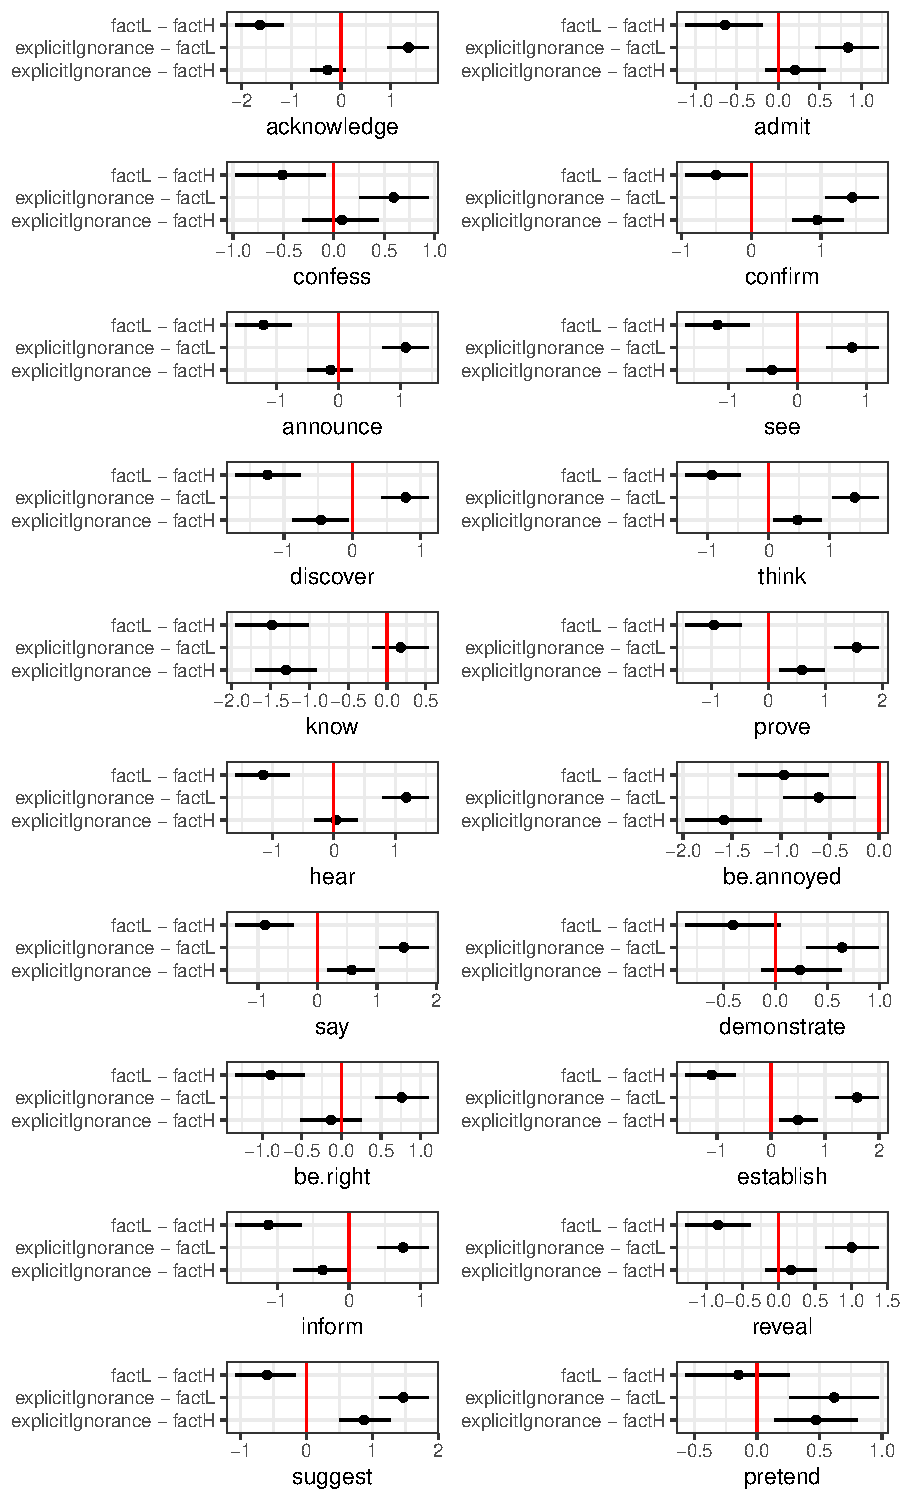
\includegraphics[width=.8\textwidth]{../../results/main/13explicitIgnorance/graphs/context-comparisons}
\caption{.}\label{fig:comparisons2}
\end{figure}
 
\end{document}

